%
\chapter{Metodologia}
\label{chap:metodologia}

\section{Descrição do Processo} \label{sec:descricaoprocesso}

Como já mencionado no \autoref{chap:introducao}, o processo modelado
neste trabalho utilizou os dados publicados por \citeonline{Rojas2014a}. 

\subsection{Diagrama Esquemático} \label{sec:diagramaesquematico}

O reator é composto de dois leitos catalíticos, carregados de forma densa
(\emph{dense loading}). No topo de ambos os leitos há catalisador carregado de
forma solta (\emph{sock loading}). A carga é composta de gasolina de pirólise,
hidrogênio e parte do produto hidrogenado reciclado. Este último é parte da
corrente líquida oriunda de um vaso de separação, cuja carga é a corrente de
saída do reator. Parte da corrente líquida do vaso de separação também
funciona como corrente de resfriamento, que é injetada entre os dois leitos
catalíticos para controle de temperatura. Um diagrama simplificado que ilustra o
reator está na \autoref{fig:esquemareator}. A \autoref{tab:dadosreator}
apresenta as dimensões do reator.

\begin{figure}[htb]
\centering 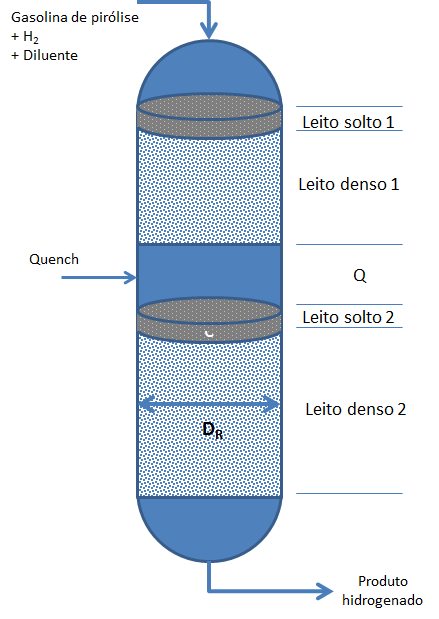
\includegraphics[scale=0.75]{images/Chap3/esquemareator.png}
\caption{Diagrama esquemático do reator \cite{Rojas2014a}.}
\label{fig:esquemareator}
\end{figure}


\begin{table}[!htb]
\begin{center}
\caption{Dados do Reator \cite{Rojas2014a}.}
\label{tab:dadosreator}
\small
\begin{tabular}{cc}
{Dimensão} & {Valor}
\\
\hline
{Diâmetro do Reator ($D_R$)} & $3,047$ m \\
{Leito Solto 1 ($L_{sl1}$)} & $0,13$ m \\
{Leito Denso 1 ($L_{dl1}$)} & $2,97$ m \\
{Leito Solto 2 ($L_{sl2}$)} & $0,38$ m \\
{Leito Denso 2 ($L_{dl2}$)} & $2,97$ m \\
{Zona de Quench ($L_{q}$)} & $1,55$ m \\
\bottomrule
\end{tabular}
\end{center}
\end{table}

\nomenclature{$L_{sl1}$}{Comprimento do leito solto 1 \nomunit{m}}
\nomenclature{$L_{dl1}$}{Comprimento do leito denso 1 \nomunit{m}}
\nomenclature{$L_{sl2}$}{Comprimento do leito solto 2 \nomunit{m}}
\nomenclature{$L_{dl2}$}{Comprimento do leito denso 2 \nomunit{m}}
\nomenclature{$L_{q}$}{Comprimento da zona de quench \nomunit{m}}

\subsection{Composição das Correntes} \label{sec:composicaocorrentes}

A composição das correntes de entrada e de quench estão na
\autoref{tab:composicao}. Para o presente trabalho, utilizou-se
apenas os valores da primeira corrida publicados por
\citeonline{Rojas2014a}, já que para essa corrida foram publicados
também dados industriais.

As propriedades termodinâmicas dos compostos $28$ e $29$ não foram
encontradas. Assim, eles foram considerados como sendo parte dos compostos
$26$ e $27$, respectivamente.

\begin{table}[!htb]
\begin{center}
\caption{Composição das correntes de entrada e de quench \cite{Rojas2014a}.}
\label{tab:composicao}
\small
\begin{tabular}{clcc}
{Identificador $i$} & {Composto} & Entrada (\% mássica) & Quench (\% mássica)
\\
\hline
1 & Hidrogênio				& $0,48$ & $0,08$ \\
2 & Metano					& $0,52$ & $0,70$ \\
3 & Etano					& $0,12$ & $0,11$ \\
4 & n-Propano				& $0,36$ & $0,27$ \\
5 & n-Butano				& $0,30$ & $0,24$ \\
6 & n-Pentano				& $5,40$ & $5,60$ \\
7 & trans-2-Penteno			& $5,30$ & $7,60$\\
8 & trans-1,3-Pentadieno	& $2,50$ & $0,23$ \\
9 & Ciclopentano			& $1,50$ & $2,60$ \\
10& Ciclopenteno			& $2,10$ & $3,00$ \\
11& Metil-1,3-Ciclopentadieno	& $1,90$ & $0,21$ \\
12& n-Hexano				& $3,30$ & $3,30$ \\
13& Metilciclopentano		& $1,60$ & $1,70$ \\
14& Metilciclopenteno		& $2,00$ & $2,60$ \\
15& 1,3-Ciclopentadieno		& $1,90$ & $0,02$ \\
16& Benzeno					& $28,90$ & $30,10$ \\
17& n-Heptano				& $2,80$ & $2,90$ \\
18& Tolueno					& $16,00$ & $16,30$ \\
19& n-Octano				& $1,30$ & $1,30$ \\
20& Etilbenzeno				& $3,40$ & $5,40$ \\
21& Estireno				& $2,00$ & $0,11$ \\
22& Xileno					& $5,40$ & $5,50$ \\
23& n-Nonano				& $0,66$ & $0,72$ \\
24& 1-Metil-3-Etilbenzeno	& $2,90$ & $3,90$ \\
25& Metilestireno			& $1,40$ & $0,31$ \\
26& Dihidrodiciclopentadieno	& $1,80$ & $3,00$ \\
27& Diciclopentadieno		& $1,80$ & $0,12$ \\
28& Metildihidrodiciclopentadieno	& $1,50$ & $2,20$ \\
29& Metildiciclopentadieno	& $0,88$ & $0,11$ \\
\bottomrule
\end{tabular}
\end{center}
Onde $i$ é o número identificador do composto na simulação a ser apresentada.
\end{table}

\nomenclature[S]{$i$}{i-ésimo componente}

\section{Premissas} \label{sec:premissas}

\subsection{Premissas adotadas por \citeonline{Rojas2014a}}
\label{sec:premissasrojas}

Antes de apresentar as premissas que nortearam o presente trabalho, vale
aqui apresentar, para efeito de comparação, as premissas utilizadas por
\citeonline{Rojas2014a}.

\begin{enumerate}
  \item O reator opera em estado estacionário e adiabaticamente.
  \item Gradientes radiais são desprezíveis.
  \item Dispersões axiais foram negligenciadas; portanto, assumiu-se o
  escoamento empistonado para ambas as fases líquida e gasosa.
  \item A fase gasosa está em excesso; dessa forma, negligenciou-se a
  resistência a transferência de massa na fase gasosa.
  \item Fator de molhamento, atividade catalítica e densidade do leito
  uniformes.
  \item A transferência de calor entre as fases e no interior das partículas de
  catalisador foram desprezadas.
  \item A entalpia de dissolução de compostos na fase gás, bem como calor de
  vaposização de líquido foram desprezadas.
  \item A região do quench é assumida como sendo um tambor flash, que atinge o
  equilíbrio instantaneamente.
  \item A corrente de saída do primeiro leito mistura-se instantaneamente com a
  corrente de quench.
  \item O reator opera em regime de bolha.
  \item Reações reversíveis e isomerizações foram negligenciadas.
  \item As reações ocorrem somente na interface líquido-sólido.
  \item A desativação catalítica foi desprezada.
\end{enumerate}

No presente estudo, algumas premissas adotadas por \citeonline{Rojas2014a} serão
alteradas, como será descrito a seguir. 

\subsection{Premissas deste trabalho} \label{sec:premissasdestetrabalho}

Como já mencionado no \autoref{chap:introducao}, um dos objetivos do presente
trabalho é avaliar algumas respostas dinâmicas ao processo proposto. Além disso,
a implementação da modelagem foi feita em \emso, software que avalia respostas
dinâmicas por concepção. Assim, convenientemente, a premissa de um reator
operando em estado estacionário foi descartada. Permanece, porém, aqui, a
premissa de que o equipamento opere de forma adiabática.

A alteração mais importante às premissas adotadas por \citeonline{Rojas2014a}, e
que representa um avaço por eles publicado, é a consideração tanto da entalpia
de dissolução do hidrogênio na fase líquida quanto da entalpida de vaporização
de líquido. Isso foi possível graças à abordagem de modelagem por células,
assunto da seção \autoref{sec:modelagemredecelulas}.

Portanto, ficam aqui definidas as seguintes premissas:

\begin{enumerate}
  \item O reator opera adiabaticamente.
  \item Gradientes radiais são desprezíveis.
  \item Dispersões axiais foram negligenciadas; portanto, assumiu-se o
  escoamento empistonado para ambas as fases líquida e gasosa.
  \item A fase gasosa está em excesso; dessa forma, negligenciou-se a
  resistência a transferência de massa na fase gasosa.
  \item Fator de molhamento, atividade catalítica e densidade do leito
  uniformes.
  \item A transferência de calor entre as fases e no interior das partículas de
  catalisador foram desprezadas.
  \item A região do \emph{quench} é assumida como sendo um tambor flash, que
  atinge o equilíbrio instantaneamente.
  \item A corrente de saída do primeiro leito mistura-se instantaneamente com a
  corrente de \emph{quench}.
  \item O reator opera em regime de borbulhamento.
  \item Reações reversíveis e isomerizações foram negligenciadas.
  \item As reações ocorrem somente na interface líquido-sólido.
  \item A desativação catalítica foi desprezada.
\end{enumerate}

Um dos motivos de se manter praticamente inalteradas as premissas adotadas por
\citeonline{Rojas2014a} foi o de realiar comparações entre os dois estudos.

Negligenciar os gradientes e dispersões de calor e massa, tanto radialmente
quanto axialmente, é uma recomendação muito comum encontrada na literatura
\cite{Ancheyta2011, Ranade2011, Froment2011} para simulações cujo objetivo é
prever o comportamento de um TBR, sob o ponto de vista de liberação de calor e
conversão das reações. Da mesma forma é a desconsideração da transferência de
calor entre as fases.

Como já mencionado no \autoref{chap:revisaobibliografica},
\citeonline{Rojas2014a} utilizaram as reações publicadas por
\citeonline{Hanika1999}. Isso pode ter motivado os autores a negligenciar a
resistencia à transferência de massa na fase gasosa.

As premissas assumidas para a região de \emph{quench} são bastante razoáveis, já
que normalmente os projetistas de reatores TBR desejam a corrente oriunda do
leito superior se misture rapidamente com a corrente de \emph{quench},
homogeneizando a carga para o segundo leito. Uma mistura inadequada entre as
correntes de entrada na região de \emph{quench} pode levar a caminhos
preferenciais e regiões de estagnação no leito inferior \cite{Ancheyta2011}.

O regime de operação por borbulhamento foi adotado para que as
equações hidrodinâmicas fossem as mesmas utilizadas por \citeonline{Rojas2014a}.
Contudo, uma verificação da validade dessa premissa é apresentada no
\autoref{chap:resultados}.

\section{Modelagem por Rede de Células} \label{sec:modelagemredecelulas}

Para utilizar a abordagem de modelagem por rede de células, cada leito
catalítico foi subdivido em células em seu comprimento, i.e., discretizado em
$N_{Disc}$ segumentos de leito. Cada seguimento de leito fica identificado por
um índice ($z$). A figura \autoref{fig:celula} ilustra uma célula de leito de
reator. Do ponto de vista reacional, cada célula representará um reator CSTR
associado a um tambor de flash. Nesse tambor de flash, foi assumido que o
equilíbrio termodinâmico é atingido instantaneamente.

 \begin{figure}[htb]
 \centering 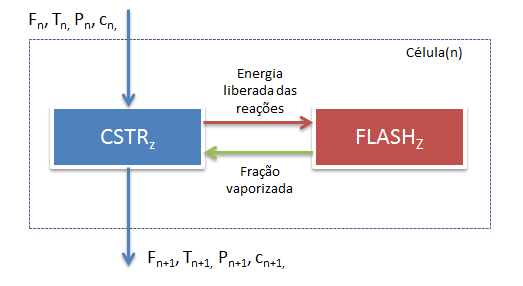
\includegraphics[scale=0.75]{images/Chap3/celula.png}
 \caption{Elemento discretizado de leito - célula}
 \label{fig:celula}
 \end{figure}

\nomenclature{$N_{Disc}$}{Número de células de um leito do reator}
\nomenclature[S]{$z$}{z-ésima célula de leito de reator}

Para a região de quench, será usado um tambor de flash, onde o equilíbrio
termodinâmico é também atingido instantaneamente. A \autoref{fig:quench} ilustra
a região de quench.

 \begin{figure}[htb]
 \centering 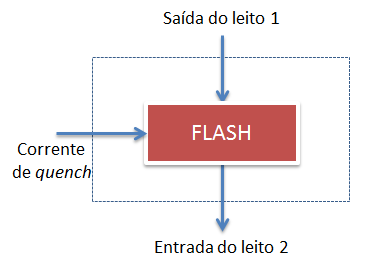
\includegraphics[scale=0.75]{images/Chap3/quench.png}
 \caption{Região de quench do reator}
 \label{fig:quench}
 \end{figure}

Com esse tipo de abordagem, foi possível considerar os efeitos termodinâmicos
ao longo do reator, como também prever a composição das fases líquida e
gasosa. As próximas seções apresentam o equacionamento construído

\section{Balanço de Massa e Energia} \label{sec:balancomassaenergia}

Normalmente, para a modelagem de TBR heterogênea, os autores que utilizam
modelos determinísticos contínuos fazem o balanço de massa para todas as
fases presentes. \citeonline{Ancheyta2011} apresenta de forma didática as
equações de balanço de massa de cada fase, explicando todos os seus termos.
Cada pesquisador, portanto, de acordo com a premissa adotada, elimina muitos dos
termos das equações de balanço, a fim simplificar o modelo e facilitar a
solução. 

Para este trabalho, contudo, foi feito o balanço de massa global, sem
distinção de fase, como mostra a \autoref{eq:balancodemassa}. Nessa equação, há
o termo de diferenciação da massa de cada componente no tempo. Isso
foi feito para permitir estudar respostas dinâmicas do processo.

\begin{equation}
F_zC_{i,z} - F_{z+1}C_{i,z+1} + \displaystyle\sum_{j=1}^{N_{reac}}
\nu_{i,j}r_{j,z} \dfrac{W}{N_{Disc}}
\label{eq:balancodemassa}
\end{equation}

onde $N_{Disc}$ é o número de células de um leito, $N_{reac}$ é o número total
de reações, $\nu_{i,j}$ é o coeficiente do componente $i$ na reação $j$, $F$ é a
vazão molar total e $W$ é a massa total de catalisador presente no leito.


É importante ressaltar que, da forma como a \autoref{eq:balancodemassa} está
escrita, a massa contida em cada célula é uma grandeza extensiva. 

\section{Cinética das Reações} \label{sec:cineticadasreacoes}

\section{Termodinâmica} \label{sec:termodinamica}

\section{Hidrodinâmica} \label{sec:hidrodinamica}

incluir cálculo de porosidade, balanço de "espaço", que está no livro do
Ancheyta, pg 131/132)

\section{Implementação em \emso} \label{sec:implementacao}






